\chapter{Graphs}

A graph is a set of vertices $V$ and edges $E$.  An edge is a pair of
vertices which are said to be connected.  For example:
%
\begin{align*}
V &= \{ A, B, C \} \\
E &= \{ (A, B), (B, C) \}
\end{align*}

Which can be represented more visually:

{
  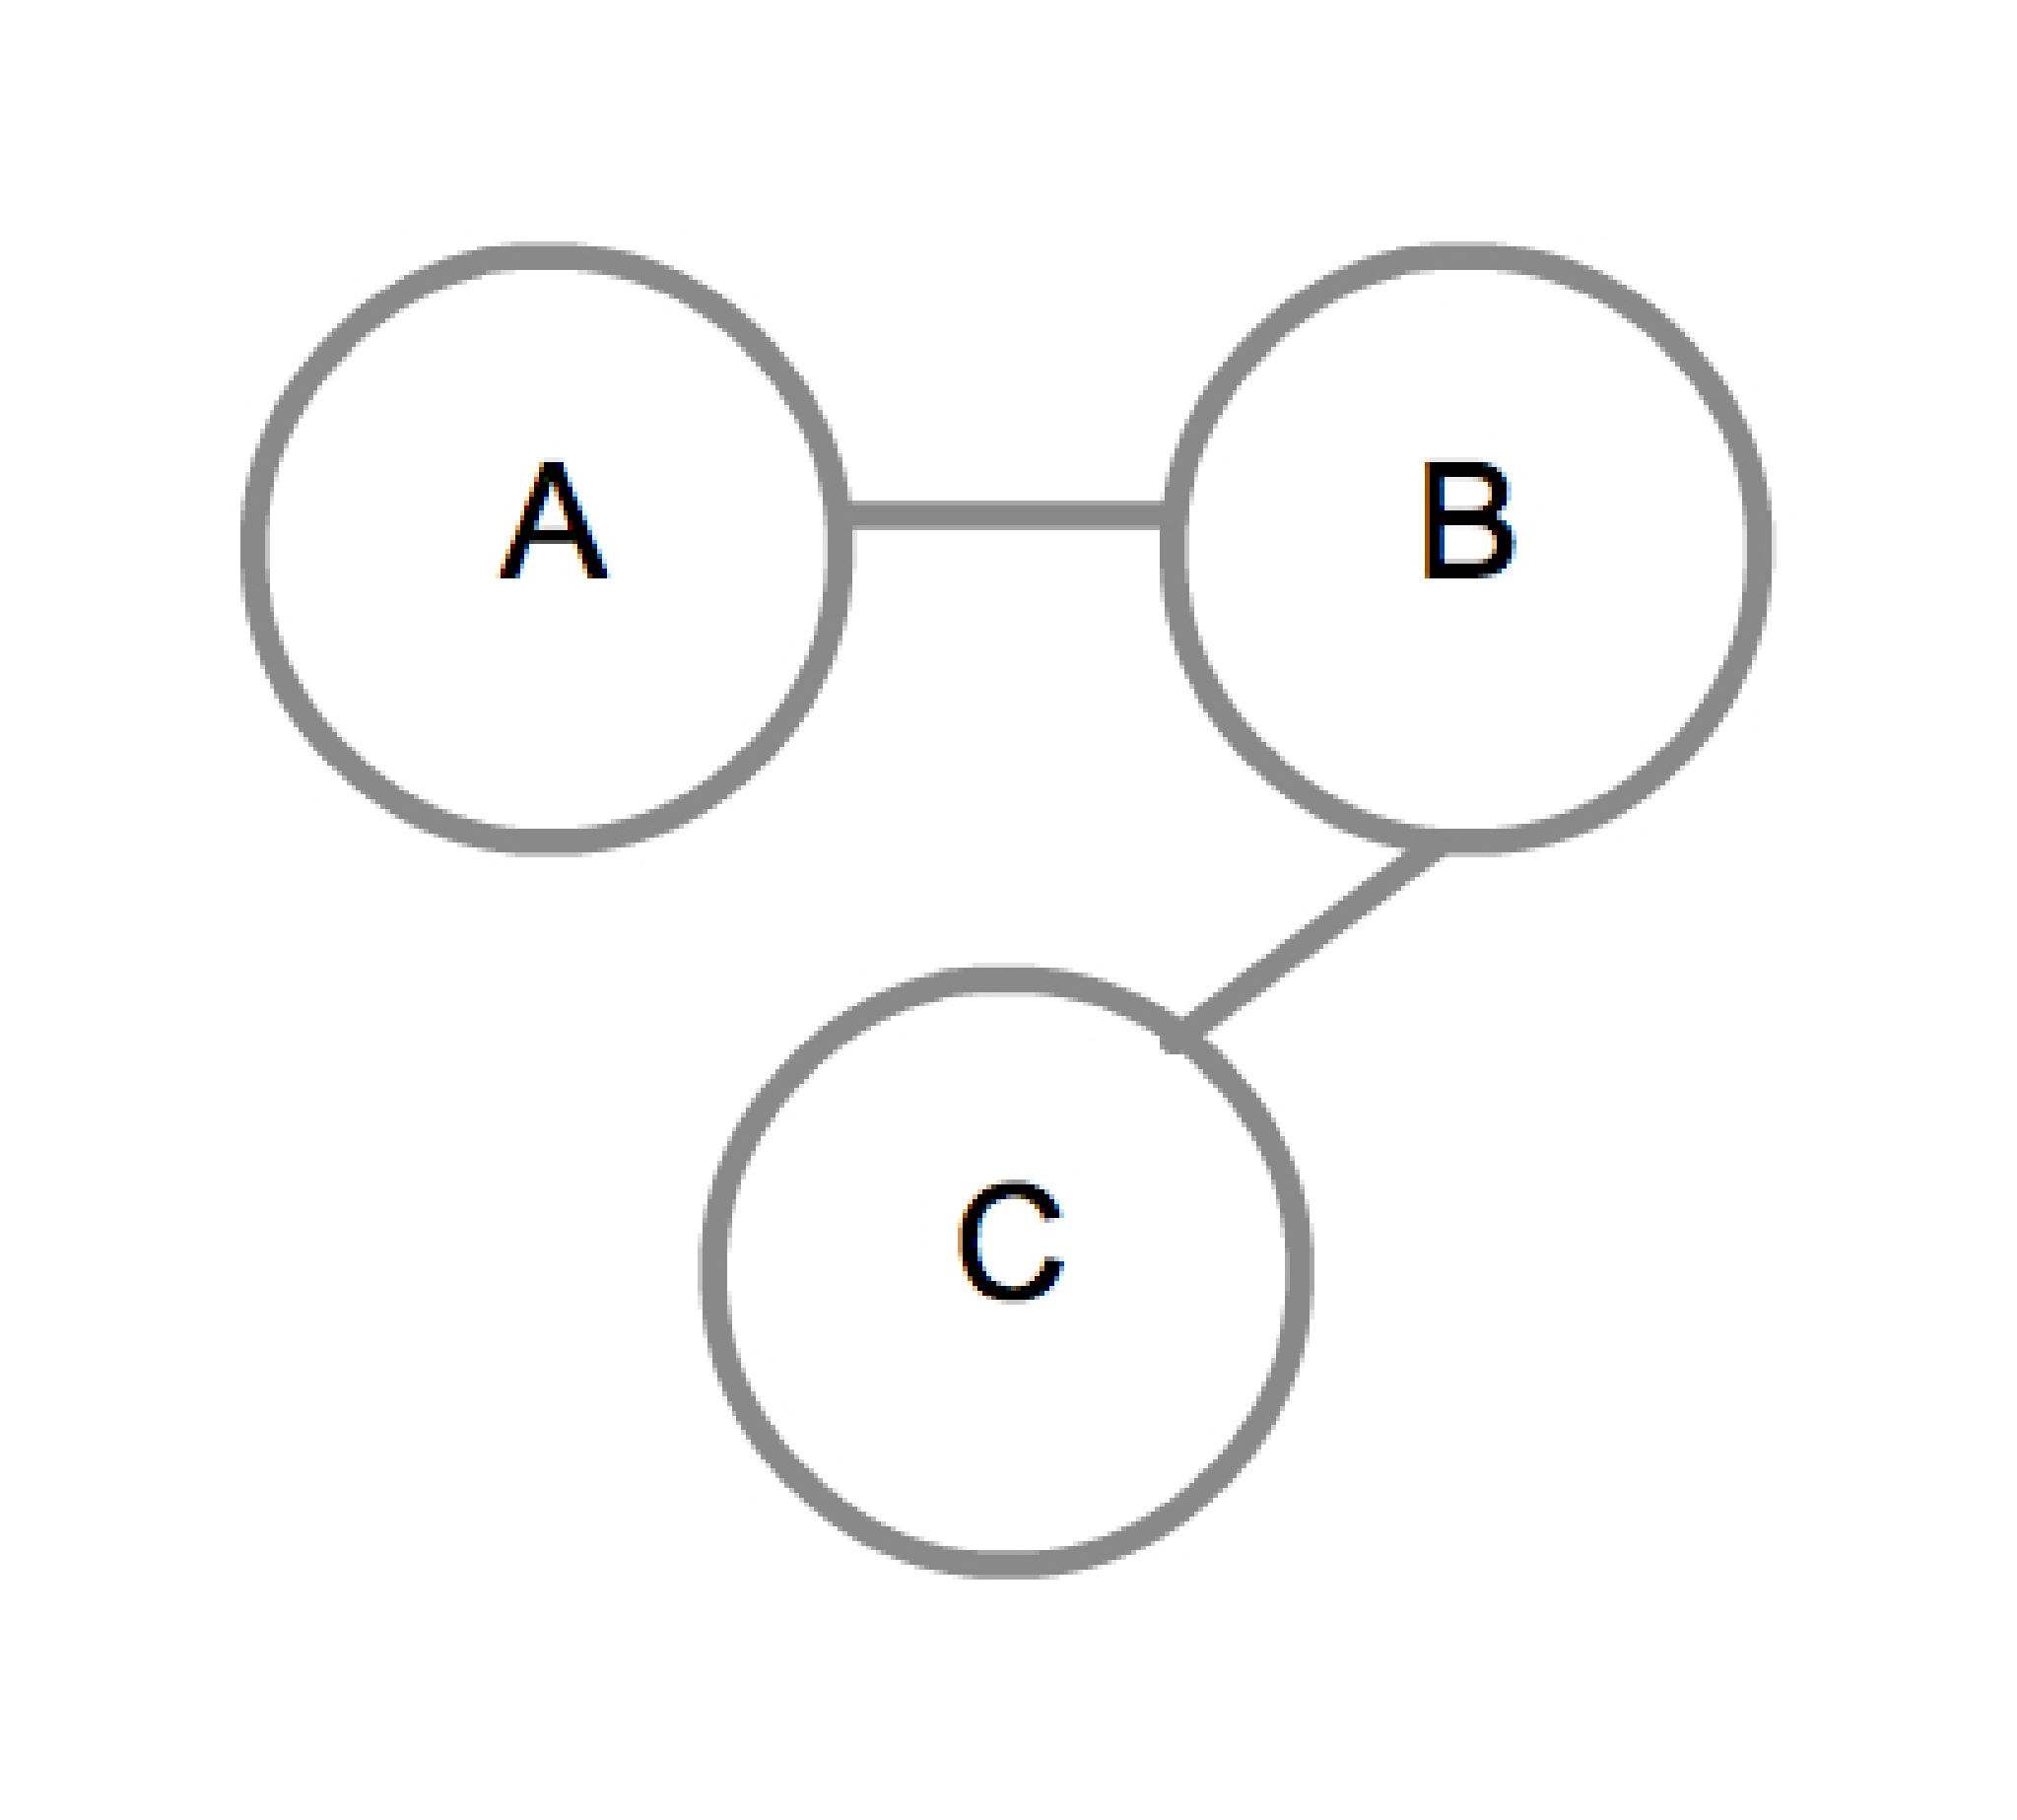
\includegraphics[scale=0.2]{SimpleGraph}
  %\caption{Demonstrates a simple graph}
  \label{fig:SimpleGraph}
}

Note that the vertices are represented by labeled circles and the
edges are represented by lines connecting vertices to one another.

The number of edges connecting a vertex $v$ is called the degree of
$v$ or $deg(v)$.  In the above example:

\begin{align*}
deg(A) = deg(C) &= 1 \\
deg(B) &= 2
\end{align*}

Sometimes an edge is directional, meaning $(A, B)$ connects $A$ to
$B$, but not $B$ to $A$.  We say such an edge is incoming on $B$ and
outgoing on $A$.  This is represented visually by an edge with an
arrow at one end, indicating the direction:

{
  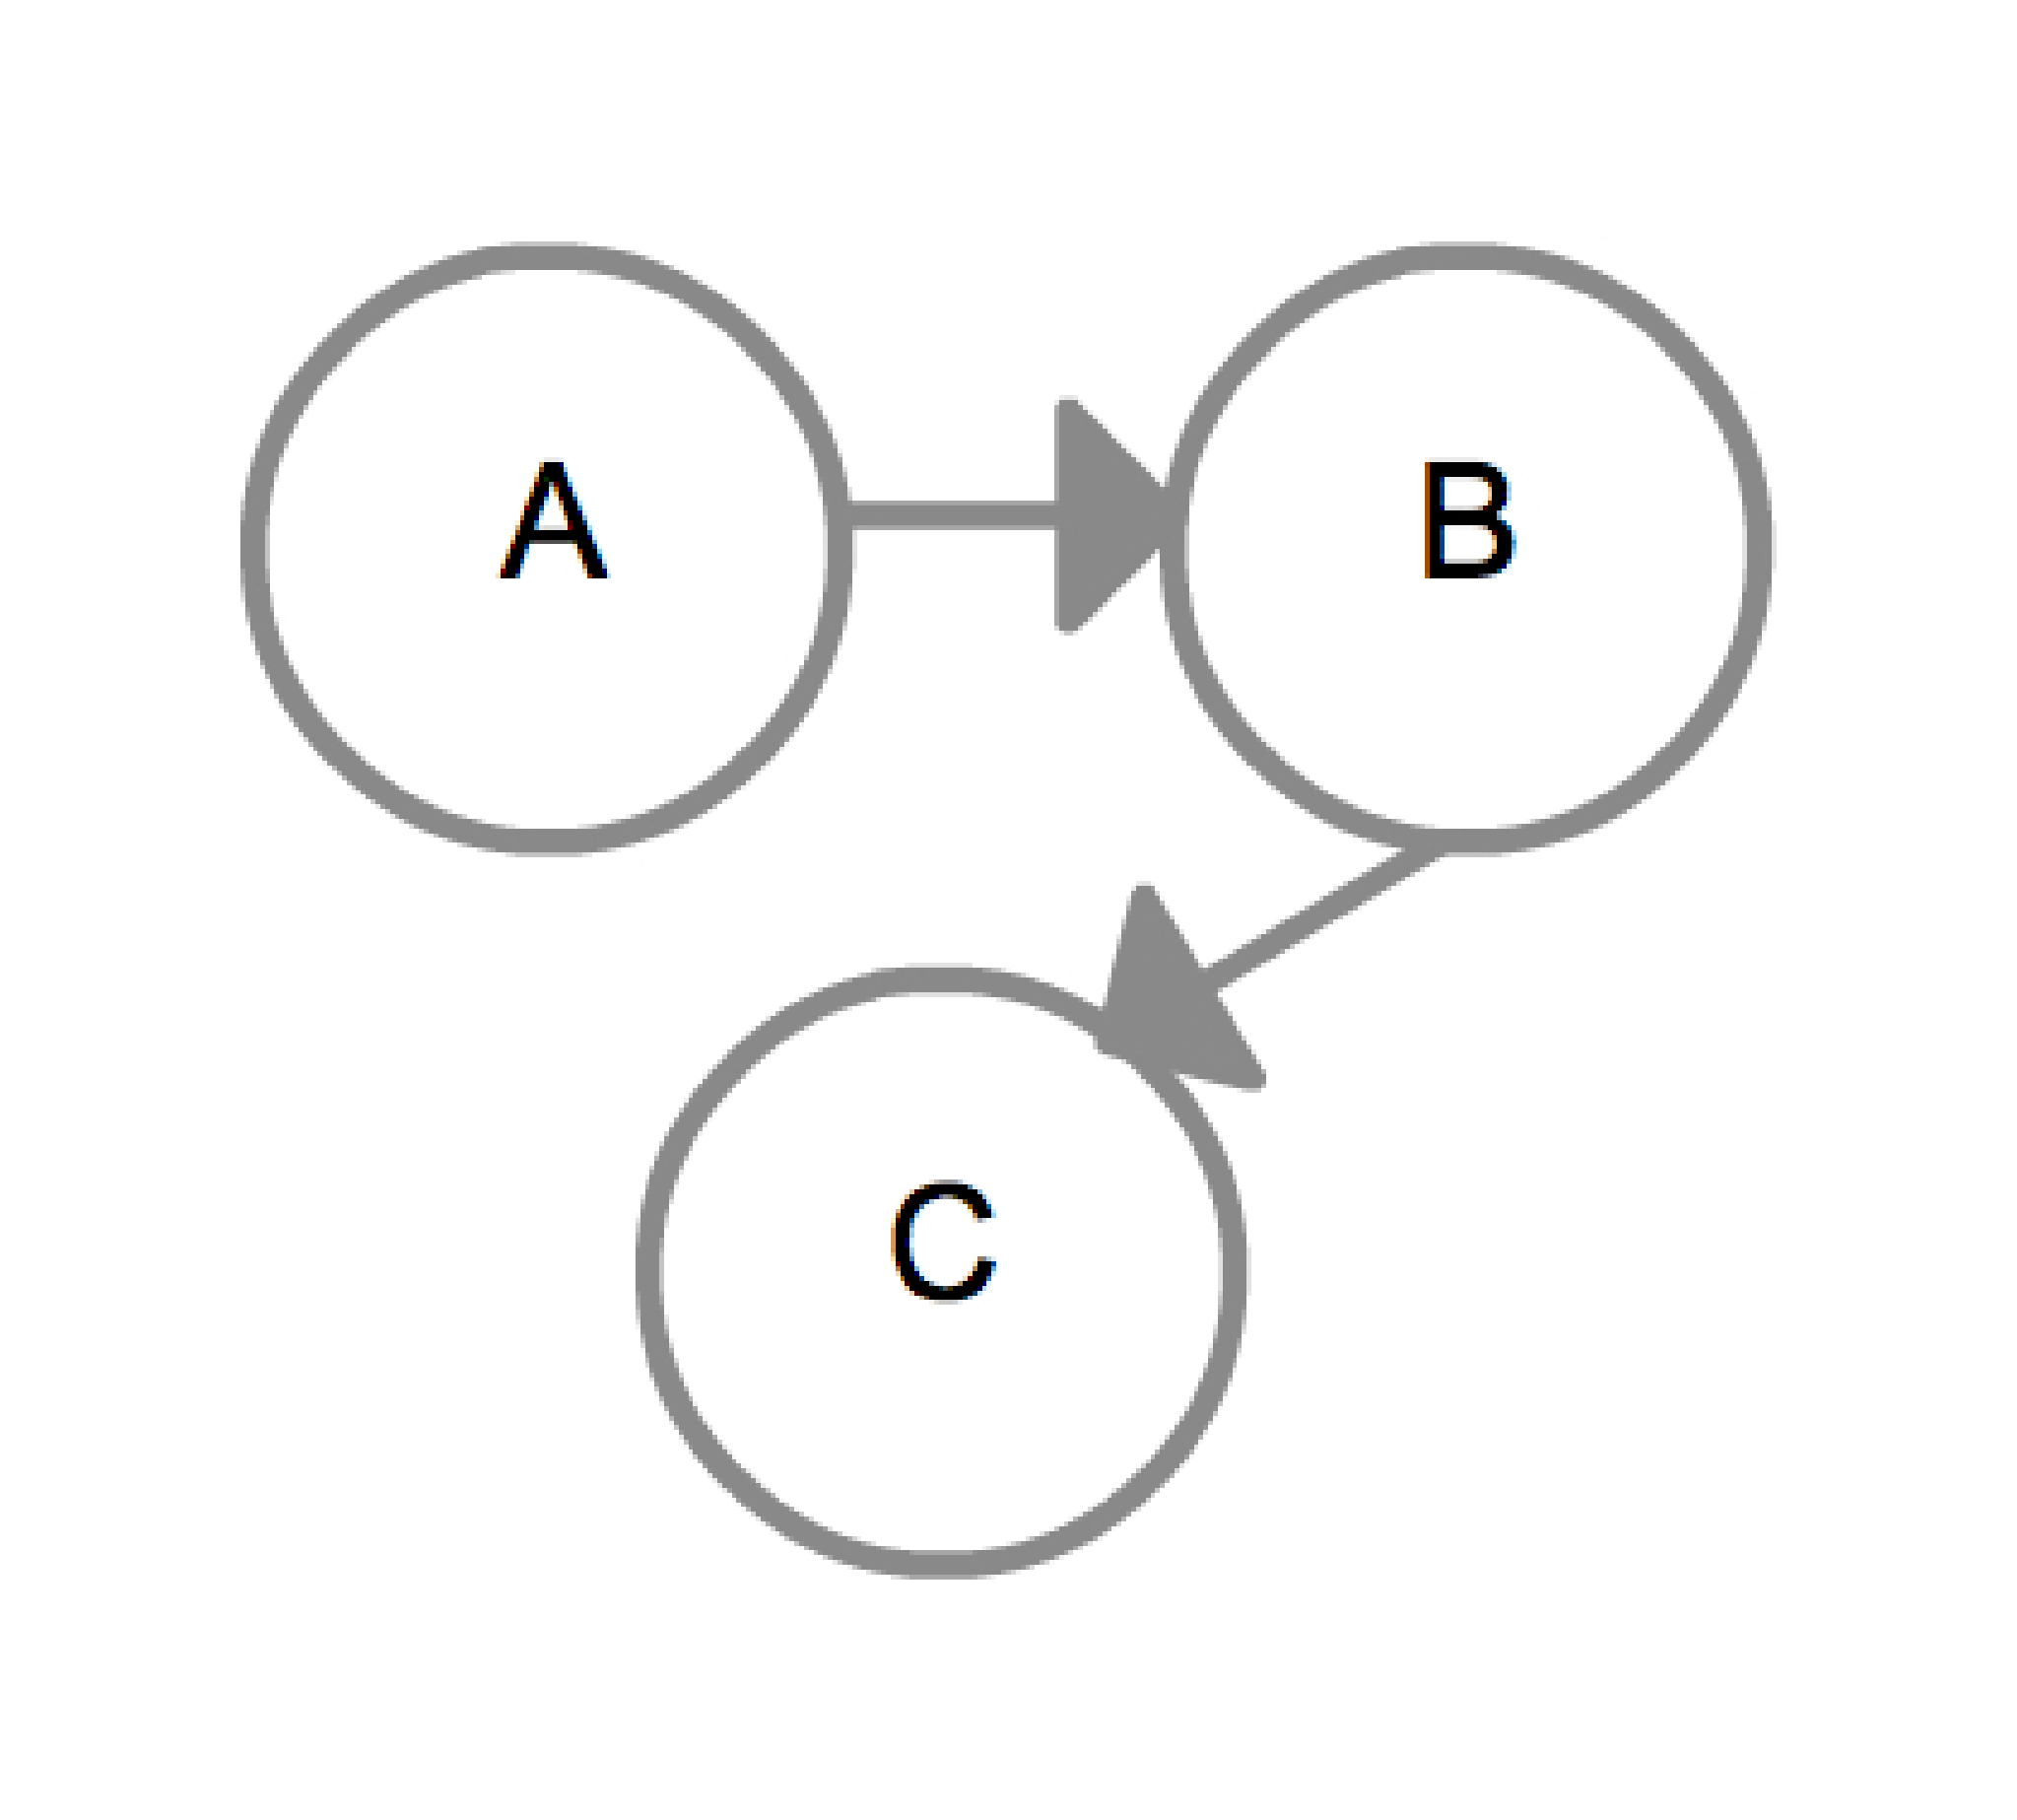
\includegraphics[scale=0.2]{DiGraph}
  %\caption{Demonstrates a directed graph}
  \label{fig:DiGraph}
}

Generally when we say graph, we mean undirected graph and will specify
directed graph or digraph.

In a digraph, the number of incoming edges of $v$ is the in-degree or
$deg^-(v)$.  Similarly, the number of outgoing edges is the
out-degree or $deg^+(v)$.

In the above example:
%
\begin{align*}
deg^+(A) = deg^+(B) &= 1 \\
deg^-(B) = deg^-(C) &= 1 \\
deg^+(C) = deg^-(A) &= 0
\end{align*}



